\chapter{Summarising the Posterior Distribution}
The posterior distribution is the full answer to any Bayesian problem. It gives
a complete description of our state of knowledge and our uncertainty about the
value(s) of unknown
parameters. From the posterior distribution, we can calculate any probability
we want. For example, if we had a posterior distribution $p(\theta|x)$ and we
wanted to know the probability that $\theta$ is greater than or equal to 100, we could do:
\begin{eqnarray}
P(\theta \geq 100 | x) &=& \int_{100}^\infty p(\theta | x) \, dx.
\end{eqnarray}
or
\begin{eqnarray}
P(\theta \geq 100 | x) &=& \sum_{100}^\infty p(\theta | x)
\end{eqnarray}
depending on whether the set of possible $\theta$ values is continuous or
discrete. We could also work out the probability of anything else.
However, the posterior distribution is sometimes too much
information for us to think about easily. Maybe a giant list of $\theta$
values and probabilities isn't easy to digest. Sometimes,
we need to {\it summarise} the posterior distribution to help us
communicate our results with others. A giant Bayes' Box (or a million MCMC
samples of the parameter, we'll see that later), might technically
contain everything we want, but it's not easy to talk about.

For example, say you were trying to estimate
a parameter, and a colleague asked you to state your uncertainty about the
parameter. Well, your posterior distribution might be complicated. It might
have bumps and wiggles in it, or some other kind of structure. If there were
two or more unknown parameters, there might be dependence in the posterior
distribution. In some cases there might even me multiple separate peaks!
Figure~\ref{fig:complicated_posterior} shows an example of what a complicated
posterior distribution might look like. If this was your result, your colleague
might not care about all the little wiggles in this plot. They just want to know
the ``big picture'' of your results.
\begin{figure}[h!]
\begin{center}
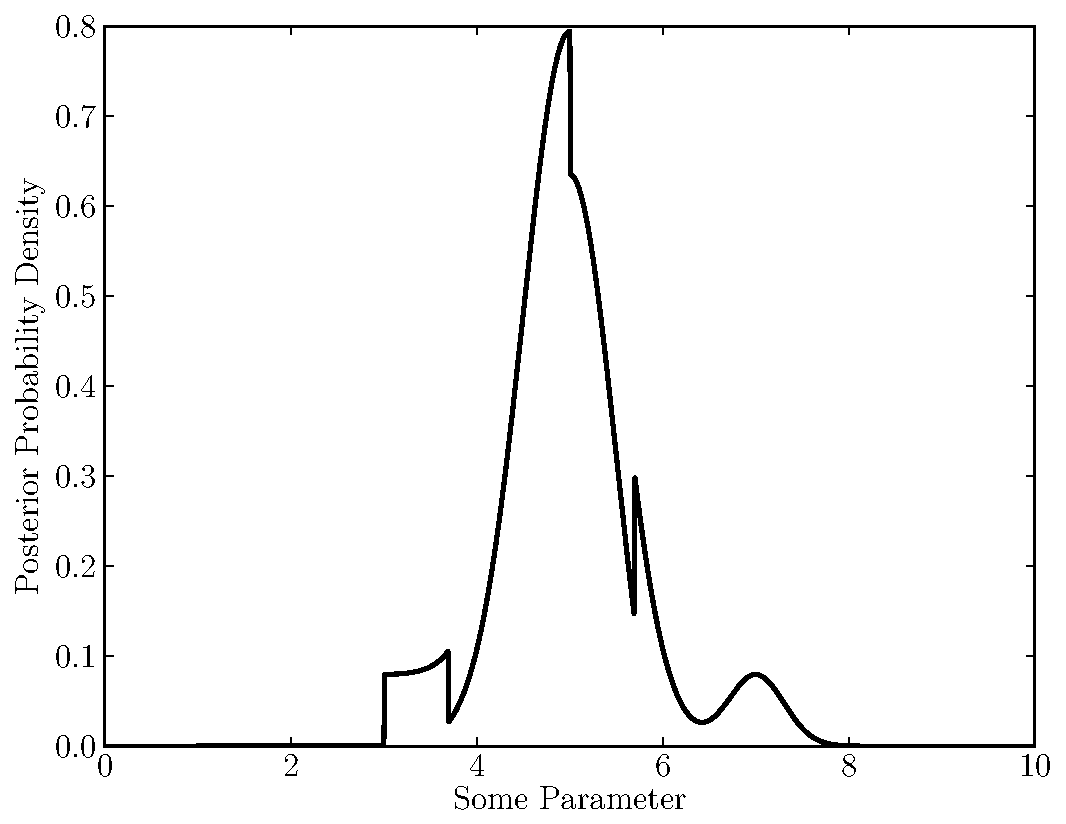
\includegraphics[scale=0.6]{Figures/complicated_posterior.pdf}
\caption{A complicated posterior distribution. When communicating with others,
it is often useful to summarise the posterior distribution by a few numbers. In
this case, something like ``distance = $5 \pm 1$'' might be a useful summary.
\label{fig:complicated_posterior}}
\end{center}
\end{figure}

The idea of summarising the posterior distribution is very closely related to
the idea of summarising a data set, that you have probably encountered when you
studied descriptive statistics.
\begin{framed}
{\bf In descriptive statistics, you often make summaries of a complex data set
(e.g. the mean and the standard deviation) so that you can communicate about
the data set in a concise way. In Bayesian statistics, you often do a similar
thing, but instead of giving a concise description of the {\it data}, you give a
concise description of the {\it posterior distribution}.}
\end{framed}

\section{Point Estimates}
A ``point estimate'' refers to a single number guess for the value of a parameter.
If you have several parameters, a point estimate would be a single guess for the
value of each parameter (like a single point in a multidimensional space).
If you look at the
posterior distribution plotted in Figure~\ref{fig:complicated_posterior}, you
can see that the true value of the parameter is probably somewhere around 5,
but with some uncertainty. If you were to provide a single number as a guess of
the parameter, you would probably say something close to 5. In classical statistics, a
single number guess is called an ``estimate'', and a rule for generating such
guesses is called an ``estimator''. Estimates are usually written by putting a
little hat over the name of the parameter. So, by looking at the plot of the
posterior, you could give an estimate like this:
\begin{eqnarray}
\hat{\theta} = 5.
\end{eqnarray}
But there are better things you could do than just looking at the plot, and I'd bet you know some of them
from previous statistics courses. Here are three methods you could use to
choose a point estimate using the posterior distribution: the posterior mean
(the expectation value of the parameter), the posterior median
(the value that divides the probability
in half), and the posterior mode (the value where the posterior distribution has its
peak). In our illustrative example, the values of these three point estimates
are:
\begin{eqnarray}
\hat{\theta} &=& 4.988 \textnormal{ (the posterior mean)}\\
\hat{\theta} &=& 4.924 \textnormal{ (the posterior median)}\\
\hat{\theta} &=& 4.996 \textnormal{ (the posterior mode)}
\end{eqnarray}
In this example, there's not much of a difference between these three methods.
But in other situations, they can be quite different (this usually happens if
the posterior distribution is skewed, or has multiple modes: you may notice a
strong analogy between this topic and descriptive statistics). Is there a way
to say which one is the {\it best}? It turns out that there is, but that
depends on what you mean by ``best''.

Before we get on to the formal ways of deciding what is a good estimate, I will
just mention a very common method that is widely used. If the posterior distribution
looks even vaguely like a normal distribution, it is common to summarise it like
this:
\begin{eqnarray}
\theta = \textnormal{posterior mean }\pm\textnormal{posterior standard deviation}.
\end{eqnarray}
In my own research I use this kind of summary frequently.

\subsection{A Very Brief Introduction to Decision Theory}
Decision theory is a very important topic. In this course we will use a
{\it tiny} amount of it. Just enough to solve the problem of ``which point
estimate is best?''. If you think about it, this is a bit of a weird question.
Obviously, the best point estimate is the true value. Of course it is, how could it
be otherwise? Our only problem is that we can't actually implement this suggestion.
We don't know the true value, we only have the posterior distribution
(which is based on all the evidence we have), so we have to do 
the best we can with that. To think about which decision is the best,
the first thing we should do is think
about what decisions are {\it possible}. For estimating a single parameter, any
real number is a possible guess.

The key idea in decision theory is the concept of {\it utility}, and the related
concept of {\it loss} (loss is just negative utility). Utility is
a numerical measure of how good it would be if a certain outcome came true.
Conversely, loss is a measure of how bad it would be if a certain outcome
came true.
Utilities are often subjective (not unlike prior probabilities), but in some
applications utility can be more concrete. For example, in betting or investment
decisions the utility can be measured in dollars. The problem with utility is
that we have uncertainty about what is going to happen, or about what is true,
so we can't just choose the decision that gives us the greatest utility. Instead
we will use our posterior probabilities, and choose the decision that gives us
the maximum possible {\it expected value} of the utility.

Imagine that we were estimating a parameter $\theta$ and we wanted to give a
point estimate $\hat{\theta}$. One idea for what the utility or loss might be is the
{\it quadratic} loss function, which is given by
\begin{eqnarray}
L(\theta, \hat{\theta}) = \left(\hat{\theta} - \theta\right)^2.
\end{eqnarray}
This thing inside the parentheses is the difference between our point estimate
and the true value. This formula says that if our point estimate is off by 2,
that is four times as bad as if we were off by 1. If we were off by 10, that is
100 times as bad as if we were off by 1, due to the squaring that is occurring.

Here is the proof. The expected value of the loss is
\begin{eqnarray}
\mathds{E}\left[L(\theta, \hat{\theta})\right] =
\int p(\theta|x)(\hat{\theta} - \theta)^2 \, d\theta
\end{eqnarray}
Since we are summing (integrating) over all possible true $\theta$ values, this
thing is only a function of our estimate $\hat{\theta}$. To minimise a function
of one variable, you differentiate it and then set the derivative to zero.
The derivative is
\begin{eqnarray}
\frac{d}{d\hat{\theta}}\mathds{E}\left[L(\theta, \hat{\theta})\right] &=&
\int p(\theta|x)\frac{d}{d\hat{\theta}}(\hat{\theta} - \theta)^2 \, d\theta \\
&=& \int p(\theta|x)2(\hat{\theta} - \theta) \, d\theta
\end{eqnarray}
Setting this equal to zero and then solving for $\hat{\theta}$ gives the final
result:
\begin{eqnarray}
\hat{\theta} &=& \int \theta p(\theta|x) \, d\theta.
\end{eqnarray}
That is, the best estimate, by the criterion of minimising expected loss (when
the loss function is quadratic), is just the posterior mean.

Note that I didn't verify that $\hat{\theta}$ minimises the expected loss
(setting the derivate to zero would also find a maximum). To check
that it really does minimise the expected loss, you can calculate the second
derivate and see that it is
positive. But that's not really needed, it would be pretty bizarre of the
posterior mean was the {\it worst} estimate!

\subsection{Linear Loss}
It may be the case that the quadratic loss/utility is not a reasonable model
for the consequences of an incorrect estimate. Another plausible form for the loss
function is the {\it linear} loss. This looks like:
\begin{eqnarray}
L(\hat{\theta}, \theta) &=& |\hat{\theta} - \theta|
\end{eqnarray}
With this assumption, the ``badness'' of an incorrect estimate is proportional
to how far the estimate is from the true value. If the estimate is twice as
far from the true value, it is twice as bad. We will not prove it (although you
are welcome to derive this yourself), but if the loss function is of this type
then the best estimate is the posterior median, which is the value of $\hat{\theta}$
for which $P(\theta \leq \hat{\theta}) = P(\theta > \hat{\theta}) = 0.5$.

\subsection{Linear Loss}
It may be the case that the quadratic loss/utility is not a reasonable model
for the consequences of an incorrect estimate. Another plausible form for the loss
function is the {\it linear} loss. This looks like:
\begin{eqnarray}
L(\hat{\theta}, \theta) &=& |\hat{\theta} - \theta|
\end{eqnarray}
With this assumption, the ``badness'' of an incorrect estimate is proportional
to how far the estimate is from the true value. If the estimate is twice as
far from the true value, it is twice as bad. We will not prove it (although you
are welcome to derive this yourself), but if the loss function is of this type
then the best estimate is the posterior median.

\subsection{All-or-nothing Loss}
The third kind of loss function we will look at is the ``all-or-nothing'' loss.
This is a good model for the situation where you need your estimate to be
completely correct, and if it isn't correct, then it is irrelevant how far your
estimate was from the true value. All incorrect estimates are equally bad.
The all-or-nothing loss looks like:
\begin{eqnarray}
L(\hat{\theta}, \theta) = \left\{
\begin{array}{lr}
1, & \hat{\theta} = \theta\\
0, & \textnormal{otherwise.}
\end{array}
\right.
\end{eqnarray}

If this seems true, it seems like you better make your chances as high as
possible, which means just choosing $\hat{\theta}$ to be the most probable value,
i.e. the posterior mode. This intuition is correct. With all-or-nothing loss,
the best estimate is the posterior mode.

\subsection{Invariance of Decisions}
You may be wondering about the definitions of our loss functions. For example,
we defined the quadratic loss as $(\hat{\theta} - \theta)^2$, but what if we
instead defined it as $3(\hat{\theta} - \theta)^2 + 5$ instead? Would our
best decision change? Luckily, the answer is no. The decision (estimate) that
minimises the expected value of a loss function $L$ also minimises the expected
value of a different loss function $aL + b$ where $a$ is any positive number
and $b$ is any other number.
For the mathematicians, the optimal decision is invariant under positive affine
transformations of the utility or loss function. Phew!

\subsection{Computing Point Estimates from a Bayes' Box}
The posterior mean is straightforward. It's the expectation value of the parameter
using the posterior distribution. In R, the code is:
\begin{framed}
\begin{verbatim}
post_mean = sum(theta*post)
\end{verbatim}
\end{framed}
You should also know how to compute this manually from a Bayes' Box, using a
calculator.

The posterior mode is also fairly straightforward. First, we can find the
highest probability in the Bayes' Box. Then we find the values of the parameter
that correspond to this probability.
\begin{framed}
\begin{verbatim}
highest_probability = max(post)
post_mode = theta[post == highest_probability]
\end{verbatim}
\end{framed}
In the case of a tie, {\tt post\_mode} might be a vector, indicating
that there isn't a single mode.

The posterior median is a little harder. We need to find the $\theta$ value
that has 50\% of the probability to the left and 50\% of the probability to the
right. Note that this isn't precisely defined in some cases, particularly with
discrete distributions. For example, if $\theta$ could be 1, 2, or 3, and the
probabilities of these were 0.3, 0.6, and 0.1, then what is the median? It is
not entirely clear.


\subsection{Computing Point Estimates from Samples}
When we use MCMC and JAGS, the output is not a vector of parameter values and
another vector of probabilities. Instead, we'll have just a vector of parameter
values, and no corresponding probabilities. The vector of parameter values is
meant to be a random sample of values drawn from the posterior distribution.
It's like saying ``here's a bunch of guesses for the parameter'', and any
region where there are a lot of guesses is considered to be a region with high
probability.

When we have samples instead of an exhaustive list of parameter values and
probabilities, the methods for computing the summaries are different. For a
parameter called $\theta$, the methods for computing the summaries are given
below.

\begin{framed}
\begin{verbatim}
# Posterior mean using samples
post_mean = mean(theta)
# Posterior mode using samples
# post_mode = ??? (this can't be done easily with samples!)
# Posterior median using samples
sorted = sort(theta)
post_mode = sorted[0.5*length(theta)]
\end{verbatim}
\end{framed}


\section{Credible Intervals}

\subsection{Computing Credible Intervals from a Bayes' Box}


\subsection{Computing Credible Intervals from Samples}


\section{Confidence Intervals}
In previous stats courses you have probably come across the concept of a
{\it confidence interval}. A confidence interval is a concept in classical
statistics that is somewhat similar to a credible interval in Bayesian statistics.
When people calculate confidence intervals, they usually want to be
able to say that they are 95\% sure that the parameter is in that interval,
given the data. This is what Bayesian credible intervals do, but {\it it is not
what classical confidence intervals do}!

Luckily, a lot of the time, the classical and the Bayesian methods for making
intervals will actually give the same interval. But this isn't always the case!
In lectures we will study an example where the Bayesian credible interval and
the classical confidence interval give completely different results. Here is
a teaser figure:

\begin{figure}[ht!]
\begin{center}
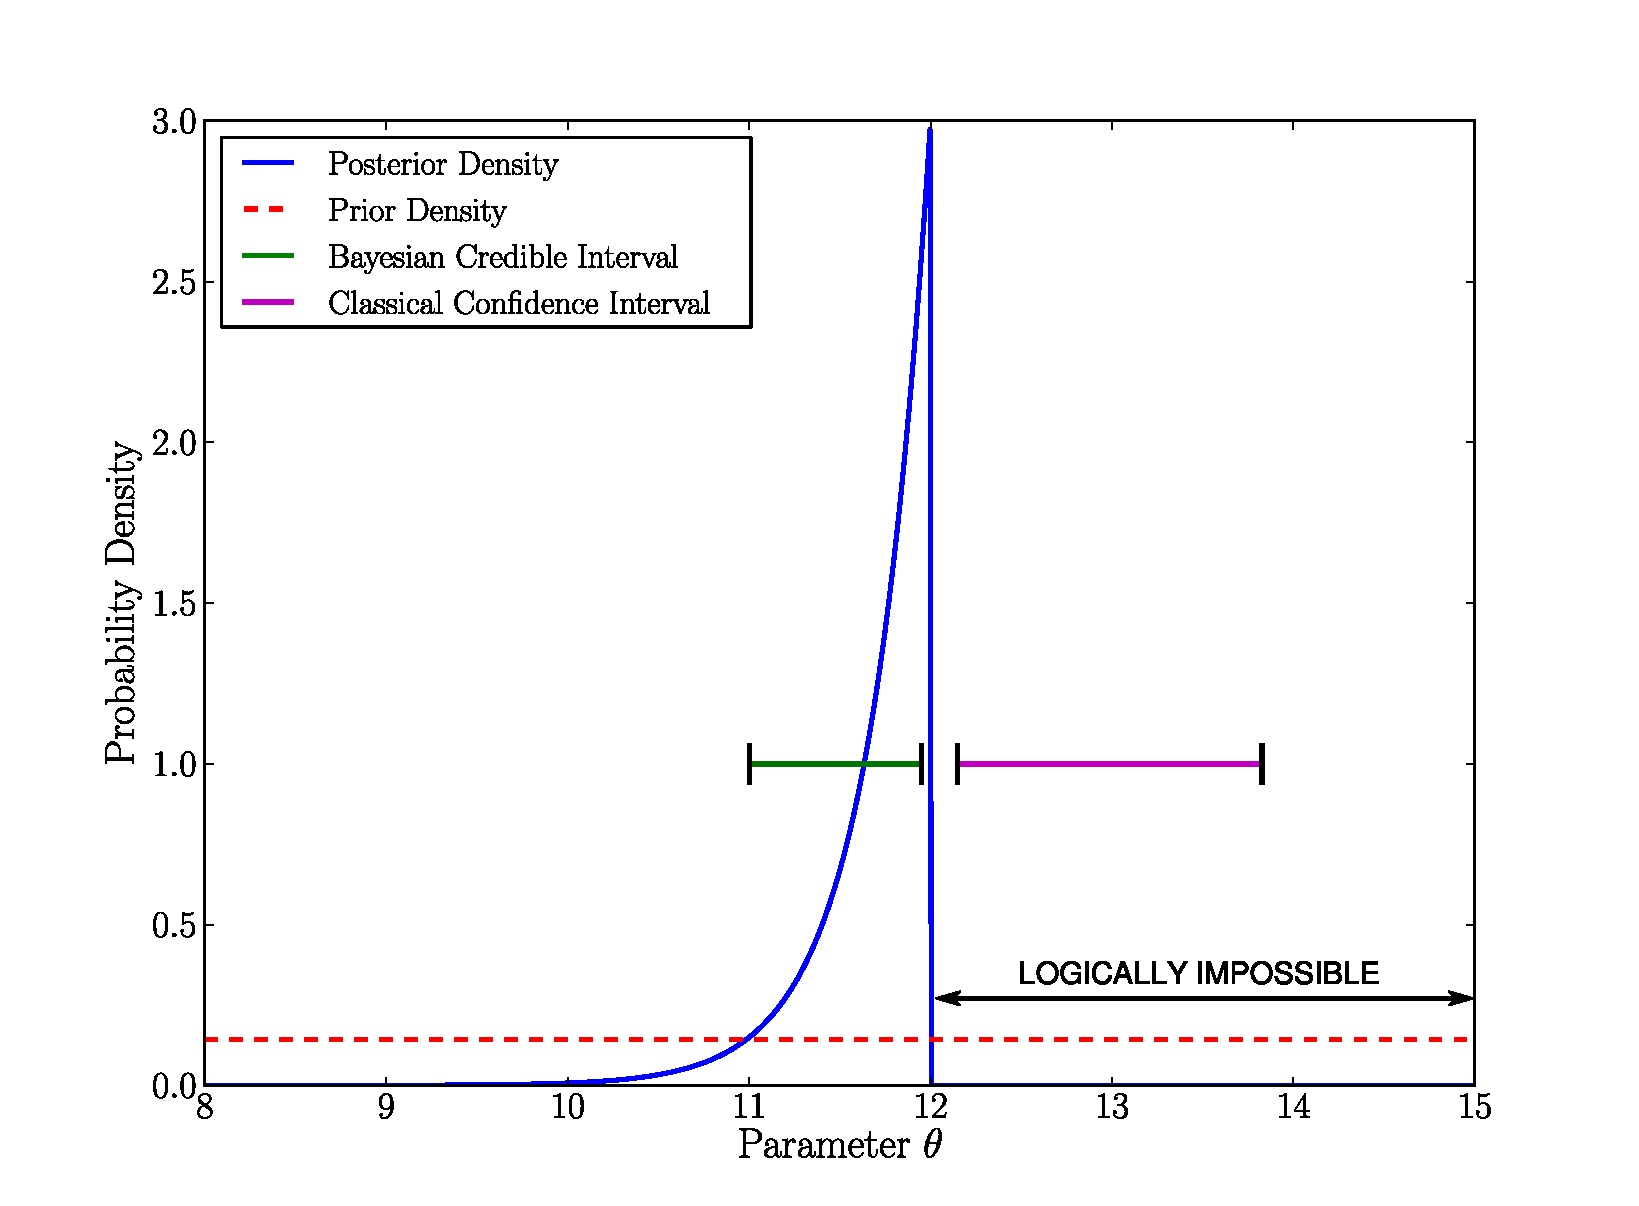
\includegraphics[scale=0.5]{Figures/jaynes.pdf}
\caption{\label{fig:jaynes}}
\end{center}
\end{figure}

